\chapter{Analisi di funzioni}
\thispagestyle{chapterInit}
\section{Notazione asintotica}
    \subsection{Definizioni}
        Si rimanda al \hyperref[sec:notazioneAsintotica]{sezione 1.2} per le definizioni di $O$, $\Omega$ e $\Theta$.
\section{Proprietà della notazione asintotica}
    \subsection{Regola Generale}
        Da qui si prende in considerazione la seguente espressione polinomiale:
        $$
            f(n) = a_kn^k + a_{k-1}n^{k-1} + \ldots + a_1n + a_0, \quad a_k > 0 \Rightarrow f(n) = \Theta(n^k)
        $$
        \paragraph{Limite Superiore} $ \exists c>0, \exists m\geq 0: f(n)\leq cn^k,\forall n\geq m $
            $$
                \begin{aligned}
                    f(n)=&a_kn^k + a_{k-1}n^{k-1} + \ldots + a_1n + a_0 \\
                    \leq& a_kn^k + \left|a_{k-1}\right|n^{k-1} + \ldots + \left|a_1\right|n + \left|a_0\right| \\
                    \leq& a_kn^k + \left|a_{k-1}\right|n^k + \ldots + \left|a_1\right|n^k + \left|a_0\right|n^k \\
                    =& (a_k + \left|a_{k-1}\right| + \ldots + \left|a_1\right| + \left|a_0\right|)n^k \quad& \forall n\geq 1\\
                    \stackrel{?}{\leq}& cn^k
                \end{aligned}
            $$
            questa è vera per $ c\geq \left(a_k + \left|a_{k-1}\right| + \ldots + \left|a_1\right| + \left|a_0\right| \right) >0$ e per $m=1$
        \paragraph{Limite Inferiore} $ \exists d > 0, \exists m\geq 0: f(n)\geq dn^k,\forall n\geq m $
            $$
                \begin{aligned}
                    f(n)=&a_kn^k + a_{k-1}n^{k-1} + \ldots + a_1n + a_0 \\
                    \geq& a_kn^k - \left|a_{k-1}\right|n^{k-1} - \ldots - \left|a_1\right|n - \left|a_0\right| \\
                    \geq& a_kn^k - \left|a_{k-1}\right|n^k - \ldots - \left|a_1\right|n^k - \left|a_0\right|n^k \\
                    =& (a_k - \left|a_{k-1}\right| - \ldots - \left|a_1\right| - \left|a_0\right|)n^k \quad& \forall n\geq 1\\
                    \stackrel{?}{\geq}& dn^k
                \end{aligned}
            $$
            questa è vera se: $ d\leq a_k - \frac{\left|a_{k-1}\right|}{n} - \ldots - \frac{\left|a_1\right|}{n} - \frac{\left|a_0\right|}{n} >0 \Leftrightarrow n>\frac{\left|a_{k-1}\right| + \ldots + \left|a_1\right| + \left|a_0\right|}{a_k} $     
        \subsubsection{Casi Particolari}
            \paragraph{Complessità di $ f(n) = 5 $}
                $$
                    \begin{aligned}
                        f(n) = 5 \geq c_1n^0 \Rightarrow c_1\leq 5 \\
                        f(n) = 5 \leq c_2n^0 \Rightarrow c_2\geq 5 \\
                        \Rightarrow f(n) = \Theta(n^0) = \Theta(1)
                    \end{aligned}
                $$
            \paragraph{Complessità di $ f(n) = 5 + \sin(n) $}
                La complessità di calcolo di $ f(n) $ è $ \Theta(1) $, in quanto $ \sin(n) $ è una funzione oscillante tra $ -1 $ e $ 1 $, quindi $ 5 + \sin(n) $ oscilla tra $ 4 $ e $ 6 $.

                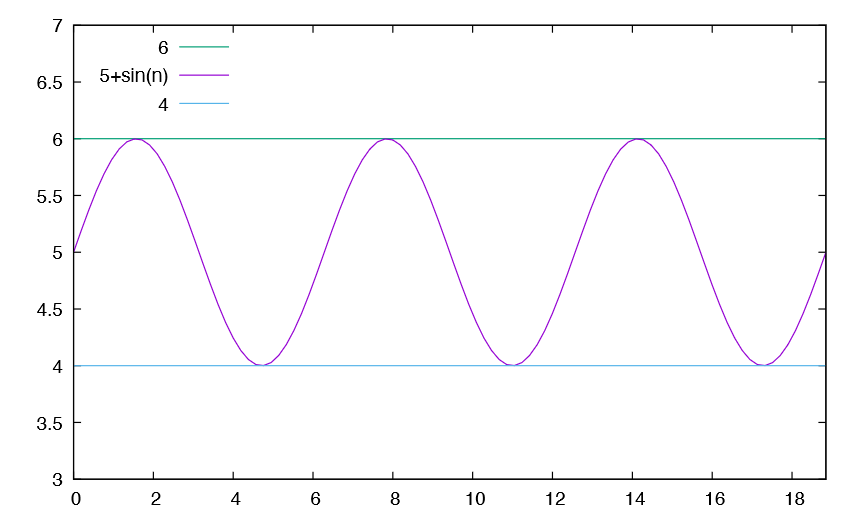
\includegraphics[scale=0.5]{02/graficoFsin.png}
    \subsection{Proprietà delle notazioni}
        \subsubsection{Dualità}
            $ f(n) = O(g(n)) \Leftrightarrow g(n) = \Omega(f(n)) $
            \begin{proof}
                $$
                    \begin{aligned}
                        f(n) = O(g(n)) \Leftrightarrow & f(n) \leq cg(n), \forall n\geq m \\
                        \Leftrightarrow & g(n) \geq \frac1cf(n), \forall n\geq m \\
                        \Leftrightarrow & g(n) \geq c'f(n), \forall n\geq m, c'=\frac1c \\
                        \Leftrightarrow & g(n) = \Omega(f(n))
                    \end{aligned}
                $$
            \end{proof}
        \subsubsection{Eliminazione di costanti}
            $$
                \begin{aligned}
                    f(n) &= O(g(n)) \Leftrightarrow af(n)=O(g(n)), \forall a>0 \\
                    f(n) &= \Omega(g(n)) \Leftrightarrow af(n)=\Omega(g(n)), \forall a>0 \\
                \end{aligned}
            $$
            \begin{proof}                
                $$
                    \begin{aligned}
                        f(n)=O(g(n)) \Leftrightarrow & f(n)\leq cg(n), \forall n\geq m \\
                        \Leftrightarrow & af(n)\leq acg(n), \forall n\geq m,\forall a>0 \\
                        \Leftrightarrow & af(n)\leq c'g(n), \forall n\geq m,c'=ac>0 \\
                        \Leftrightarrow & af(n)=O(g(n)), \forall a>0
                    \end{aligned}
                $$
            \end{proof}
        \subsubsection{Sommatoria (sequenza di algoritmi)}
            $$
                \begin{aligned}
                    f_1(n) = O(g_1(n)), f_2(n) = O(g_2(n)) \Rightarrow f_1(n) + f_2(n) = O(\max(g_1(n),g_2(n)))\\
                    f_1(n) = \Omega(g_1(n)), f_2(n) = \Omega(g_2(n)) \Rightarrow f_1(n) + f_2(n) = \Omega(\max(g_1(n),g_2(n)))
                \end{aligned}
            $$
            \begin{proof}[Dimostrazione (Lato $ O $).]
                $$
                    \begin{aligned}
                        f_1(n) = O(g_1(n)) \land f_2(n) = O(g_2(n)) & \Rightarrow \\
                        f_1(n) \leq c_1g_1(n) \land f_2(n) \leq c_2g_2(n) & \Rightarrow \\
                        f_1(n) + f_2(n) \leq c_1g_1(n) + c_2g_2(n) & \Rightarrow \\
                        f_1(n) + f_2(n) \leq \max\{c_1,c_2\}(2\cdot \max(g_1(n),g_2(n))) & \Rightarrow \\
                        f_1(n) + f_2(n) = O(\max(g_1(n),g_2(n))) &
                    \end{aligned}
                $$
            \end{proof}
        \subsubsection{Prodotto (cicli annidati)}
            $$
                \begin{aligned}
                    f_1(n) = O(g_1(n)), f_2(n) = O(g_2(n)) \Rightarrow f_1(n) \cdot f_2(n) = O(g_1(n) \cdot g_2(n))\\
                    f_1(n) = \Omega(g_1(n)), f_2(n) = \Omega(g_2(n)) \Rightarrow f_1(n) \cdot f_2(n) = \Omega(g_1(n) \cdot g_2(n))
                \end{aligned}
            $$
            \begin{proof}
                $$
                    \begin{aligned}
                        f_1(n) = O(g_1(n)) \land f_2(n) = O(g_2(n)) & \Rightarrow \\
                        f_1(n) \leq c_1g_1(n) \land f_2(n) \leq c_2g_2(n) & \Rightarrow \\
                        f_1(n)\cdot f_2(n) \leq c_1c_2g_1(n)g_2(n) &
                    \end{aligned}
                $$
        \end{proof}
        \subsubsection{Simmetria}
            $$
                f(n) = \Theta(g(n)) \Leftrightarrow g(n) = \Theta(f(n))
            $$
            \begin{proof}
                Grazie alla proprietà della dualità, si ha che:
                $$
                    \begin{aligned}
                        f(n) = \Theta(g(n)) &\quad \Rightarrow \quad f(n) = O(g(n)) \Rightarrow g(n) = \Omega(f(n))\\
                        f(n) = \Theta(g(n)) &\quad \Rightarrow \quad f(n) = \Omega(g(n)) \Rightarrow g(n) = O(f(n))
                    \end{aligned}
                $$
            \end{proof}
        \subsubsection{Transitività}
            $$
                \begin{aligned}
                    f(n) = O(g(n)), g(n) = O(h(n)) \Rightarrow f(n) = O(h(n))
                \end{aligned}
            $$
            \begin{proof}
                $$
                    \begin{aligned}
                        f(n) = O(g(n)) \land g(n) = O(h(n)) & \Rightarrow \\
                        f(n) \leq c_1g(n) \land g(n) \leq c_2h(n) & \Rightarrow \\
                        f(n) \leq c_1c_2h(n) & \Rightarrow \\
                        f(n) = O(h(n)) &
                    \end{aligned}
                $$
            \end{proof}
    \subsection{Altre funzioni di costo}
        \subsubsection{Logaritmi v/s funzioni lineari}
            \paragraph{Proprietà dei Logaritmi}
                Vogliamo provare che $ \log(n) = O(n) $. Dimostriamo per induzione che
                $$
                    \exists c>0,\exists m\geq 0:\log n\leq cn,\forall n\geq m\qquad \text{definizione di }O
                $$
                \begin{proof}
                    \begin{basecase} ($ n=1 $):
                        $ \log 1 = 0 \leq \stackrel{c}0\cdot \stackrel{n}1 = 0 $
                    \end{basecase}
                    \begin{inductiveipothesis}
                        Sia $ \log k \leq ck, \forall k\leq n $.
                    \end{inductiveipothesis}
                    \begin{inductivecase}
                        Dimostriamo la proprietà per $ n+1 $:
                        $$
                            \begin{aligned}
                                \log(n+1) \leq & \log(n+n) = \log 2n & \forall n\geq 1 \\
                                = & \log 2 + \log n \qquad & \log ab = \log a + \log b \\
                                = & 1 + \log n & \log 2 = 1 \\
                                \leq & 1 + cn & \text{per induzione} \\
                                \stackrel{?}{\leq} & c(n+1) & \text{Obbiettivo} \\
                                1+cn\leq c(n+1) \Leftrightarrow & c\geq 1
                            \end{aligned}
                        $$
                    \end{inductivecase}
                \end{proof}
        \subsection{Giocando con le espressioni}
            \paragraph{Es 1}
                È vero che $ \log_a n = \Theta(\log n) $?

                Si: $ \log_a n = (\log_a 2) \cdot (\log_2 n) = \Theta(\log n) $
            
            \paragraph{Es 2}
                È vero che $ \log n^a = \Theta(\log n) $, per $ a>0 $?

                Si: $ \log n^a = a\log n = \Theta(\log n) $
            
            \paragraph{Es 3}
                È vero che $ 2^{n+1} = \Theta(2^n) $?

                Si: $ 2^{n+1} = 2\cdot 2^n = \Theta(2^n) $
            \paragraph{Es 4}    
                È vero che $ 2^{n} = \Theta(3^n) $?

                Ovviamente $ 2^{n} = O(3^n) $

                Ma: $ 3^{n} = \left(\frac32\cdot 2\right)^n=\left(\frac32\right)^n\cdot 2^n: $ Quindi non esiste $ c > 0 $ tale per cui $ \left(\frac32\right)^n\cdot 2^n\leq c2^n $, quindi $ 2^n \neq O(3^n) $
    \subsection{Classificazione delle funzioni}
        È possibile definire un ordinamento delle principali classi estendendo le relazioni che abbiamo dimostrato:
        
        Per ogni $r<s,h<k,a<b$:
        $$
            o(1) \subset O(\log^r n) \subset O(\log^s n) \subset O(n^h) \subset O(n^h \log^r n ) \subset O(n^h \log^s n) \subset O(n^k) \subset O(a^n) \subset O(b^n)
        $$
\section{Ricorrenze}
    \subsection{Introduzione}
        \paragraph{Equazioni di ricorrenza} Quando si calcola la complessità di un algoritmo ricorsivo, questa viene espressa tramite un'\textbf{equazione di ricorrenza}, ovvero una formula definita in maniera ricorsiva.
            \subparagraph{MergeSort}
                $$
                    T(n) = \begin{cases}
                        1 & \text{se } n=1 \\
                        2T\left(\frac{n}{2}\right) + n & \text{se } n>1
                    \end{cases}
                $$
        \paragraph{Forma Chiusa} L'obbiettivo è quello di ottenere, quando possibile, una \textbf{formula chiusa} che rappresenti la classe di complessità della funzione.
            \subparagraph{MergeSort}
                $$ 
                    T(n) = \begin{cases}
                        T(\lfloor n/2 \rfloor) + T(\lceil n/2 \rceil) + \Theta(n) & n > 1 \\
                        \Theta(1) & n \leq 1
                    \end{cases} \Longrightarrow T(n) = \Theta(n\log n)
                $$
    \subsection{Metodo dell'albero di ricorsione, o per livelli}
        \paragraph{Introduzione} "Srotoliamo" la ricorrenza in un albero i costi ai vari livelli della ricorsione.
        \subsubsection{Esempio 1}
            $$
                T(n)=\begin{cases}
                    T(n/2) + b & n>1 \\
                    c & n\leq 1
                \end{cases}
            $$
            È possibile risolvere questa ricorrenza nel modo seguente:
            $$
                \begin{aligned}
                    T(n) = & b + T(n/2) \\
                    = & b + b + T(n/4) \\
                    = & b + b + b + T(n/8) \\
                    = & \ldots \\
                    = & \underbrace{b+b+\ldots+b}_{\log n} + T(1) \\
                \end{aligned}
            $$
            Assumiamo per semplicità che $ n=2^k $. $ T(n) = b\log n + c = \Theta(\log n) $
        \subsubsection{Esempio 2}
            $$
                T(n)=\begin{cases}
                    4T(n/2) + n & n>1 \\
                    1 & n\leq 1
                \end{cases}
            $$
            È possibile risolvere questa ricorrenza nel modo seguente:
            $$
                \begin{aligned}
                    T(n)=&\cancel{n\sum_{j=0}^{\log(n-1)} 2^j} &\underbrace{+4^{\log n}}_{\text{somma degli }T(1)}\\
                    \Rightarrow &\underbrace{n\cdot \frac{\overbrace{2^{\log n }}^{n\text{ per prop. log.}}-1}{2-1}}_{\stackrel{\text{usando: }}{\forall x\neq 1:\sum_{j=0}^kx^j=\frac{x^{k+1}-1}{x-1}}}&+4^{\log n}\\
                    =& n(n-1)&+4^{\log n}\\
                    =& n^2-n&\overbrace{+n^2}^{\text{cambiamento di base}}\\
                    =& 2n^2-n = \Theta(n^2)
                \end{aligned}
            $$
        \subsubsection{Esempio 3}
        $$
            T(n)=\begin{cases} 4T(n/2) + n^3 & n>1 \\ 1 & n\leq 1 \end{cases}
        $$
        Da questa equazione notiamo che il primo livello ha costo $ n^3 $, il secondo $ 4\left(\frac{n}{2}\right)^3 $ il terzo $ 4^2\left(\frac{n}{2^2}\right)^3 $ e così via. Quindi possiamo scrivere la sommatoria:
        $$
            \begin{aligned}
                T(n)=& n^3 + 4\left(\frac{n}{2}\right)^3 + \ldots + 4^{\log n-1}\left(\frac{n}{2^{\log n-1}}\right)^3 &+ 4^{\log n} \\
                =& \sum_{i=0}^{\log n-1}4^i\left(\frac{n}{2^i}\right)^3 & + 4^{\log n} \\
                =& n^3\sum_{i=0}^{\log n-1}\left(\frac{2^{2i}}{2^{3i}}\right) & + 4^{\log n} \\
                =& n^3\sum_{i=0}^{\log n-1}\left(2^{2i-3i}\right) & + 4^{\log n} \\
                =& n^3\sum_{i=0}^{\log n-1}\left(2^{-1\cdot i}\right) & + 4^{\log n} \\
                =& n^3\sum_{i=0}^{\log n-1}\left(\frac{1}{2}\right)^i & \overbrace{+n^2}^{\text{cambiamento di base}} \\
                \leq & n^3\sum_{i=0}^{\infty}\left(\frac{1}{2}\right)^i & +n^2 \\
                =& n^3\cdot \overbrace{\frac{1}{1-\frac{1}{2}}}^{\text{usando: }\forall x,|x|\leq 1:\sum_{i=0}^{\infty}x^i=\frac{1}{1-x}} & +n^2 \\
                =& 2n^3 + n^2
            \end{aligned}
        $$
        \footnote{In quanto la sommatoria tende a crescere allora abbiamo potuto sostituire $ \log n $ con $ \infty $ e modificare il segno di uguaglianza con quello di $ \leq $ in quanto la sommatoria verso l'infinito converge è più grande di quella finita}\newline
        Abbiamo dunque dimostrato che $ T(n) \leq 2n^3 + n^2 = O(n^3) $ però non possiamo, tramite la dimostrazione precedente, dire che $ T(n) = \Theta(n^3) $ in quanto siamo passati ad una disequazione. In questo particolare caso d'altra parte possiamo notare che $ T(n) \geq n^3 $ il che ci porta ad affermare che $ T(n) = \Omega(n^3) $ e quindi $ T(n) = \Theta(n^3) $. 
    \subsection{Metodo di sostituzione}
        \paragraph{Introduzione} È il metodo in cui si cerca di \textbf{indovinare} (\textbf{guess}) la soluzione e si prova a dimostrarla per \textbf{induzione}.
        \subsubsection{Primo esempio}
            $$ T(n) = \begin{cases} T(\lfloor n/2 \rfloor) + n & n>1 \\ 1 & n\leq 1 \end{cases} $$
            Notiamo come il costo dei vali livelli sia $ n + n/2 + n/4 + \ldots $. Dunque possiamo ipotizzare di poter scrivere:
            $$
                \begin{aligned}
                    T(n)=& n \cdot \sum_{i=0}^{\log n}\left(\frac{1}{2}\right)^i\\
                    \leq & n \cdot \sum_{i=0}^{\infty}\left(\frac{1}{2}\right)^i\\
                    = & n \cdot \underbrace{\frac{1}{1-\frac{1}{2}}}_{\text{usando }\forall x,|x| < 1: \sum_{i=0}^{\infty}x^i=\frac{1}{1-x}}\\
                    = & 2n
                \end{aligned}
            $$
            \footnote{Abbiamo potuto usare il $ \leq $ in quanto la sommatoria in questione all'infinito è sempre maggiore di quella finita e ci stiamo calcolando il costo massimo}
            \paragraph{Limite superiore}
                Tentiamo quindi ora di dire che $ T(n) = O(n) $:
                \subparagraph{Caso Base} $ T(1) = 1 \stackrel{?}{\leq} 1 \cdot c \Leftrightarrow \forall c\geq 1 $
                \subparagraph{Passo Induttivo} Dimostriamo la disequazione per $T(n)$
                $$
                    \begin{aligned}
                        T(n) = & T(\lfloor n/2 \rfloor) + n \\
                        \leq & \overbrace{c\lfloor n/2 \rfloor}^{\text{ipotizzato} O(n)} + n \\
                        \leq & c\cdot\overbrace{n/2}^{\text{intero inferiore}} + n \\
                        = & n(c/2 + 1) \\
                        \stackrel{?}{\leq} & cn \\
                        \Leftrightarrow & c/2 + 1 \leq c \Leftrightarrow c\geq 2
                    \end{aligned}
                $$
                
                Dunque abbiamo provato che: $ T(n) \leq cn $, nel caso base $ c\geq 1 $ e nel passo induttivo $ c\geq 2 $. In quanto deve valere per entrambi i casi allora il primo valore utile di $ c $ è $2$, avendo provato che per $ n=1 $ la disequazione vale e che per tutti i successivi valori di $ n $ la disequazione vale allora possiamo dire che $ T(n) = O(n) $.
            \paragraph{Limite Inferiore}
                Tentiamo di dimostrare che $ T(n) = \Omega(n) $:
                \subparagraph{Caso Base} Dimostriamo che $ T(1) = 1 \stackrel{?}{\geq} 1\cdot d \Leftrightarrow \forall d\leq 1 $
                \newpage % Per evitare che il passo induttivo vada a capo
                \subparagraph{Passo Induttivo} Dimostriamo la disequazione per $ T(n) $:
                $$
                    \begin{aligned}
                        T(n) =& T(\lfloor n/2 \rfloor) + n \\
                        \geq & \overbrace{d\lfloor n/2 \rfloor}^{\text{per ipo. induttiva sostituzione}} + n \\
                        \geq & d\cdot\overbrace{\frac{n}2-1}^{\text{intero inferiore}} + n \\
                        = & \left(\frac{d}2-\frac1n+1\right)n \stackrel{?}{\geq} dn \\
                        \Leftrightarrow & \frac{d}2-\frac1n+1 \geq d \\ 
                        \Leftrightarrow & d\leq 2 - \frac2n
                    \end{aligned}
                $$

                Abbiamo quindi dimostrato che $ T(n) \geq dn $, nel caso base $ d\leq 1 $ e nel passo induttivo $ d\leq 2 - \frac2n $. In quanto deve valere per entrambi i casi allora il primo valore utile di $ d $ è $1$, avendo provato che per $ n=1 $ la disequazione vale e che per tutti i successivi valori di $ n $ la disequazione vale allora possiamo dire che $ T(n) = \Omega(n) $.
                
            \paragraph{Conclusione} Avendo provato che $ T(n) = O(n) $ e $ T(n) = \Omega(n) $ e ricordando che se $ T(n) = O(n) \land T(n) = \Omega(n) \Leftrightarrow T(n) = \Theta(n) $ concludendo che la funzione di costo di $ T(n) $ cresce in maniera lineare.
        \subsubsection{Terzo esempio - Difficoltà matematiche}
            $$
                T(n)=\begin{cases} T\left(\left\lfloor\frac{n}2\right\rfloor\right) + T\left(\left\lceil\frac{n}2\right\rceil\right) + 1 & n>1 \\ 1 & n\leq 1 \end{cases}
            $$
            \paragraph{Limite Superiore}
                Dalla seguente si può notare come il costo di ogni livello sia $ 1 $ e che il numero di livelli sia $ \log n $. Inoltre la ricorsione viene eseguita su due rami, quindi possiamo scrivere la seguente sommatoria:
                $$
                    \begin{aligned}
                        T(n)=&\sum_{i=0}^{\log n}2^i\\
                        =&1+2+4+\ldots+\frac{n}4+\frac{n}2+n \\
                        =&O(n)
                    \end{aligned}
                $$
                Proviamo ora a dimostrare che $ T(n) = O(n) $:
                \subparagraph{Passo Induttivo} Ipotizzando che $ \forall k<n:T(k)\leq ck $, dimostriamo che $ T(n)\leq cn $:
                    $$
                        \begin{aligned}
                            T(n)=&T\left(\left\lfloor\frac{n}2\right\rfloor\right) + T\left(\left\lceil\frac{n}2\right\rceil\right) + 1 \\
                            \leq & c\left\lfloor\frac{n}2\right\rfloor + c\left\lceil\frac{n}2\right\rceil + 1 \\
                            \leq & cn+1 \\
                            \stackrel{?}{\geq} & cn \Rightarrow 1\leq 0 & \text{ impossibile}
                        \end{aligned}
                    $$
                    Sebbene la dimostrazione sia fallita ma l'intuizione ci dice che $ T(n) = O(n) $

                Proviamo dunque a dimostrarlo per un \textbf{ordine inferiore}: $ cn+1\leq cn $
                \subparagraph{Passo Induttivo} Ipotizzando che $ \exists b>0,\forall k<n:T(k)\leq ck-b $ allora dimostriamo la disequazione per $T(n)$:
                    $$
                        \begin{aligned}
                            T(n)=&T\left(\left\lfloor\frac{n}2\right\rfloor\right) + T\left(\left\lceil\frac{n}2\right\rceil\right) + 1 \\
                            \leq & c\left\lfloor\frac{n}2\right\rfloor - b + c\left\lceil\frac{n}2\right\rceil - b + 1 \\
                            =& cn - 2b + 1 \\
                            \stackrel{?}{\leq} & cn - b \\
                            \Rightarrow & \cancel{cn} - 2b + 1 \leq \cancel{cn} - b \Rightarrow b\geq 1
                        \end{aligned}
                    $$
                    Dimostriamo il passo base per $ b=1 $: $ T(1) = 1 \stackrel{?}{\leq} 1\cdot c - b\Leftrightarrow \forall c\geq b+1 $
            \paragraph{Limite Inferiore} 
                Proviamo ora a dimostrare che $ T(n) = \Omega(n) $:
                \subparagraph{Passo Induttivo} Ipotizzando che $ \forall k<n:T(k)\geq dk $, dimostriamo che $ T(n)\geq dn $:
                    $$
                        \begin{aligned}
                            T(n)=&T\left(\left\lfloor\frac{n}2\right\rfloor\right) + T\left(\left\lceil\frac{n}2\right\rceil\right) + 1 \\
                            \geq & d\left\lfloor\frac{n}2\right\rfloor + d\left\lceil\frac{n}2\right\rceil + 1 \\
                            = & dn + 1 \\
                            \stackrel{?}{\geq} & dn \Rightarrow 1\geq 0 
                        \end{aligned}
                    $$ Il che è vero $ \forall d $ in quanto $ d $ è positivo per ipotesi.
                \subparagraph{Caso base} Dimostriamo la disequazione per $ T(1) $:
                    $$
                        T(1) = 1 \geq 1\cdot d \Leftrightarrow d\leq 1
                    $$Dunque abbiamo provato che $ T(n) = \Omega(n) $

                Avendo dimostrato in precedenza che $ T(n) = O(n) $ e $ T(n) = \Omega(n) $ possiamo concludere che $ T(n) = \Theta(n) $ e quindi la funzione di costo cresce linearmente.
    \subsection{Metodo dell'esperto, o delle ricorrenze comuni}
        \paragraph{Riccorenze comuni} Esiste un'ampia classe di ricorrenze che si risolvono facilmente facendo ricorso a qualche teorema, ogni teorema è applicabile ad una particolare classe di ricorrenze.
        \subsubsection{Ricorrenze lineari con partizione bilanciata}
            \begin{theorem}
                Siano $ a,b $ costanti intere tali che $ a \geq 1 $ e $ b \geq 2 $, e esistano $c,\beta$ costanti reali tali che $ c > 0 $ e $ \beta \geq 0 $. Sia $ T(n) $ data dalla seguente relazione di ricorrenza:
                \begin{align}
                    T(n)=\begin{cases}
                        aT(n/b) + cn^\beta & n>1 \\
                        1 & n\leq 1
                    \end{cases}
                \end{align}
                Posto: $\alpha = \frac{\log a}{\log b}= \log_b a$ allora:
                \begin{align}
                    T(n)=\begin{cases}
                        \Theta(n^\alpha) & \alpha > \beta \\
                        \Theta(n^\alpha\log n) & \alpha = \beta \\
                        \Theta(n^\beta) & \alpha < \beta
                    \end{cases}
                \end{align}
            \end{theorem}
            \paragraph{Assunzioni} Assumiamo che $ n $ sia una potenza intera di $ b $, ovvero $ n=b^k, k=\log_bn $.
                \subparagraph{Influisce sul risultato?}
                    \begin{itemize}
                        \item Supponendo che l'input abbia dimensione $b^{k}+1$
                        \item Estendiamo l'input fino alla dimensione $b^{k+1}$ (\textbf{padding})
                        \item L'input è stato esteso di un fattore $b$
                        \item Il che non cambia la complessità computazionale
                    \end{itemize}
            \paragraph{Dimostrazione caso 1}
            \paragraph{Dimostrazione caso 2} $\alpha = \beta $
            \begin{proof}
                Ne segue che: $q=b^{\alpha-\beta}=1$ e dunque la funzione $T(n)$:
                \begin{align}
                    T(n)=&dn^\alpha+cb^{k\beta}\sum_{i=0}^{k-1}q^i\\
                    =&n^\alpha d+cn^\beta k \qquad & q^i=1^i=1\\
                    =&n^\alpha d+cn^\alpha k & \alpha = \beta\\
                    =&n^\alpha(d+ck)\\
                    =&n^\alpha\left[d+c\frac{\log n}{\log b}\right] & k=\log_b n
                \end{align}
            \end{proof}
            e come conseguenza $T(n)=\Theta(n^\alpha\log n)$
        \subsubsection{Ricorrenze lineari con partizione bilanciata (Estesa)}
        \begin{theorem}
            Sia $ a\geq 1, b>1, f(n) $ asintoticamente positiva e sia:
            $$
                T(n)=\begin{cases}
                    aT(n/b) + f(n) & n>1 \\
                    \Theta(1) & n\leq 1
                \end{cases}
            $$
            Sia $ \alpha = \log_b a $ si distinguono i seguenti casi:
            \begin{table}[H]
                \centering
                \begin{tabular}{|c|l c l|}
                    \hline
                    (1) & $ \exists\epsilon>0:f(n)=O(n^{\alpha - \epsilon})$ & $\Rightarrow$ & $T(n)=\Theta(n^\alpha)$ \\\hline
                    (2) & $ f(n)=\Theta(n^\alpha)$ & $\Rightarrow$ & $T(n)=\Theta(f(n)\log n)$ \\ \hline
                    (3) & $ \begin{array}{l}
                        \exists \epsilon>0:f(n)=\Omega(n^{\alpha + \epsilon}) \land\\
                        \exists c:0<c<1, \\
                        \exists m\geq 0:af(n/b)\leq cf(n),\\\forall n\geq m
                    \end{array} $ & $\Rightarrow$ & $T(n)=\Theta(f(n))$ \\\hline
                \end{tabular}
            \end{table}
        \end{theorem}